\documentclass{beamer}
\usetheme{Luebeck}
\usecolortheme{seahorse}
\usefonttheme{structurebold,serif}
\setbeamertemplate{navigation symbols}{\usebeamerfont{footline}\insertframenumber/\inserttotalframenumber}
\usepackage{luatexja-fontspec}
\setmainfont{STIX Two Text}
\setsansfont{Helvetica}
\setmonofont{Inconsolata}
\setmainjfont{YuKyo_Yoko-Medium}[BoldFont=YuKyo_Yoko-Bold]
\setsansjfont{YuGo-Medium}[BoldFont=YuGo-Bold]
\usepackage{mathtools}
\usepackage[warnings-off={mathtools-colon,mathtools-overbracket}]{unicode-math}
\unimathsetup{math-style=ISO,bold-style=ISO}
\setmathfont{STIX Two Math}
\mathtoolsset{showonlyrefs=true}
\usepackage{tikz}
\usetikzlibrary{cd}
\usepackage[mark=o]{dynkin-diagrams}

\title{Onsager代数とその周辺}
\author{宇佐見 公輔}
\date{第4回 すうがく徒のつどい}
\begin{document}
\maketitle

\begin{frame}
    \frametitle{自己紹介}

    \begin{itemize}
        \item 宇佐見 公輔(うさみ こうすけ)
        \item 本業はプログラマー
        \item 大学院で数学専攻、修士卒業後は趣味としてやっている
        \item Lie代数やその周辺を好む
    \end{itemize}

    \bigskip

    今回は一般枠の講演として応募しましたが、入門枠のほうが適切だったかもしれません。
\end{frame}

\begin{frame}
    \frametitle{今日の話}

    \begin{itemize}
        \item 背景
        \item Lie代数とその関連用語
        \item Onsager代数
        \item Onsager代数の拡張
    \end{itemize}
\end{frame}

\begin{frame}
    \frametitle{背景}

    Onsager代数は、統計力学の数理模型である2次元Ising模型の厳密解を導く際に導入された代数構造です(Onsager 1944)。これは$ℂ$上の無限次元Lie代数です。

    \bigskip

    その後、Chiral Potts模型の解法でも利用される(1980〜1990)など、他にもいくつかの数理模型の研究で用いられています。

    \bigskip

    Onsager代数の一般化もいくつか研究されており、Generalized Onsager代数、q-Onsager代数、などがあります。これらも数理物理への応用が研究されています。
\end{frame}

\begin{frame}
    \frametitle{背景}

    \begin{columns}[c]
        \begin{column}{0.7\linewidth}
            \begin{itemize}
                \item 2次元Ising模型:\(m \times n\) の格子模型
                \item 配置$s=(s_{ij})$(ここで、$s_{ij}=\pm 1$)
                \item 周期境界条件$s_{i+m,j}=s_{ij}$、$s_{i,j+n}=s_{ij}$
                \item エネルギー
                      \begin{equation}
                          E(s)=-J_1\sum_{i,j}s_{ij}s_{i+1,j}-J_2\sum_{i,j}s_{ij}s_{i,j+1}
                      \end{equation}
                \item 分配関数
                      \begin{equation}
                          Z(T)=\sum_{s}\mathrm{exp}(-βE(s))
                      \end{equation}
            \end{itemize}
        \end{column}
        \begin{column}{0.3\linewidth}
            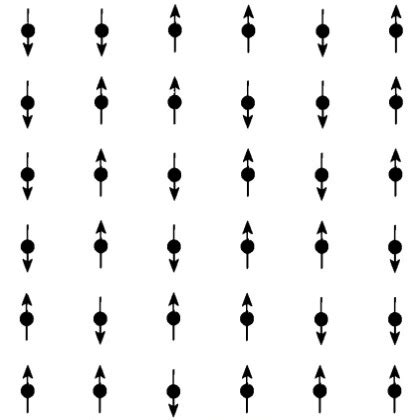
\includegraphics[width=\linewidth]{images/ising.jpeg}
        \end{column}
    \end{columns}

    \bigskip

    統計力学の模型を解くとは、$m,n→∞$のときの分配関数$Z(T)$を求めることです。
\end{frame}

\begin{frame}
    \frametitle{背景}

    2次元Ising模型の分配関数は、転送行列というものを導入することで、
    \begin{equation}
        Z(T)=\mathrm{tr}(V_1V_2)^m
    \end{equation}
    と書けます(ここで$V_1$、$V_2$は$2^n×2^n$行列)。このため、2次元Ising模型を解くことは、$V_1V_2$の固有値を求めることに帰着します。

    \bigskip

    転送行列は$V_1$と$V_2$は、ある行列$A_0$、$A_1$を用いて
    \begin{equation}
        V_1=\mathrm{exp}(K_1A_1),\quad V_2=\mathrm{exp}(-K_2^*A_0)
    \end{equation}
    と書けます。この$A_0$、$A_1$で生成されるLie代数をOnsager代数と呼びます。これを詳しく調べることで、2次元Ising模型の厳密解が得られます。
\end{frame}

\begin{frame}
    \frametitle{Lie代数の定義}

    集合$L$に、加法、スカラー倍、ブラケット積の3つの演算を考えます。
    \begin{align}
        L\times L & \to L       \\
        (x,y)     & \mapsto x+y
    \end{align}
    \begin{align}
        ℂ\times L & \to L      \\
        (α,x)     & \mapsto αx
    \end{align}
    \begin{align}
        L\times L & \to L        \\
        (x,y)     & \mapsto[x,y]
    \end{align}
\end{frame}

\begin{frame}
    \frametitle{Lie代数の定義}

    \begin{definition}[Lie代数]
        集合$L$が$ℂ$上のLie代数であるとは、以下を満たすことです。
        \begin{itemize}
            \item $L$は加法とスカラー倍で$ℂ$上のベクトル空間になる。
            \item (双線型性)$∀x,y,z∈L$、$∀α\inℂ$について
                  \begin{alignat}{2}
                      [x+y,z] & =[x,z]+[y,z], & \quad [αx,z] & =α[x,z] \\
                      [z,x+y] & =[z,x]+[z,y], & \quad [z,αx] & =α[z,x]
                  \end{alignat}
            \item (交代性)$∀x∈L$について
                  \begin{equation}
                      [x,x]=0
                  \end{equation}
            \item (Jacobi恒等式)$∀x,y,z∈L$について
                  \begin{equation}
                      [x,[y,z]]+[y,[z,x]]+[z,[x,y]]=0
                  \end{equation}
        \end{itemize}
    \end{definition}
\end{frame}

\begin{frame}
    \frametitle{Lie代数の定義}

    なお、$[x,x]=0$から
    \begin{equation}
        [x,y]=-[y,x]
    \end{equation}
    が導けます。

    \bigskip

    また、ブラケット積は結合法則$[x,[y,z]]=[[x,y],z]$を満たさず、代わりに
    \begin{equation}
        [x,[y,z]]=[[x,y],z]+[y,[x,z]]
    \end{equation}
    という関係が成り立ちます。
\end{frame}

\begin{frame}
    \frametitle{関連用語の定義}

    \begin{definition}[準同型写像]
        $L$と$M$をLie代数とします。写像$ϕ:L→M$がLie代数の準同型写像であるとは、$ϕ$が線型写像であり、$∀x,y∈L$について
        \begin{equation}
            ϕ([x,y])=[ϕ(x),ϕ(y)]
        \end{equation}
        を満たすことです。
    \end{definition}

    \begin{definition}[同型]
        Lie代数の準同型写像$ϕ:L→M$が線型同型写像であるとき、$ϕ$をLie代数の同型写像と呼びます。$L$から$M$へのLie代数の同型写像が存在するとき、$L$と$M$は同型であるといいます。
    \end{definition}
\end{frame}

\begin{frame}
    \frametitle{関連用語の定義}

    \begin{definition}[部分Lie代数]
        $L$をLie代数とします。$L$の部分集合$S$が部分Lie代数であるとは、$S$が部分ベクトル空間であり、$∀x,y∈S$について$[x,y]∈S$を満たすことです。
    \end{definition}

    \begin{definition}[イデアル]
        $L$をLie代数とします。$L$の部分集合$I$がイデアルであるとは、$I$が部分ベクトル空間であり、$∀x∈L$、$∀y∈I$について$[x,y]∈I$を満たすことです。
    \end{definition}
\end{frame}

\begin{frame}
    \frametitle{関連用語の定義}

    \begin{definition}[商Lie代数]
        $L$をLie代数、$I$をイデアルとします。商ベクトル空間$L/I$にブラケット積を$[\overline{x},\overline{y}]:=\overline{[x,y]}$で定めると、$L/I$はLie代数となります。これを商Lie代数と呼びます。
    \end{definition}

    補足:$I$が単に部分Lie代数だとブラケット積がwell-definedでないことに注意してください。
\end{frame}

\begin{frame}
    \frametitle{結合代数}

    \begin{definition}[結合代数]
        集合$A$が$ℂ$上の結合代数であるとは、加法、スカラー倍、乗法の3つの演算が定義されていて、以下の条件を満たすことです。
        \begin{itemize}
            \item $A$は加法とスカラー倍で$ℂ$上のベクトル空間になる。
            \item 乗法$A×A→A$は双線型写像となる。
            \item $A$は加法と乗法で環になる。すなわち、乗法は結合法則を満たし単位元を持つ(なお、交換法則は仮定しない)。
        \end{itemize}
    \end{definition}

    「結合代数」という言葉を使いましたが、通常はわざわざ「結合」と言わずに「代数」「多元環」と呼ばれることが多いです。今はLie代数の話をしていて結合法則を満たすことが当たり前ではないので、あえて「結合代数」と呼んでいます。
\end{frame}

\begin{frame}
    \frametitle{結合代数}

    結合代数が与えられたとき、ブラケット積を$[x,y]:=xy-yx$で定義すると、結合代数としての乗法を忘れて、加法とスカラー倍とブラケット積でLie代数となります。

    \begin{example}[行列のLie代数]
        $\mathrm{M}(n,ℂ)$を$ℂ$上の$n$次正方行列全体の集合とします。これは通常の加法、スカラー倍、乗法で結合代数です。

        $\mathrm{M}(n,ℂ)$にブラケット積を$[X,Y]:=XY-YX$で定めるとLie代数となります。これは$\mathfrak{gl}(n,ℂ)$と呼ばれます。
    \end{example}

    補足:このような結合代数とLie代数の関係から、$[x,y]=0$となることを「$x$と$y$が可換である」という言い方をします。
\end{frame}

\begin{frame}
    \frametitle{基底を使ったLie代数の表示}

    $ℂ$上のベクトル空間$L$が与えられたとして、この$L$がLie代数となるようにブラケット積を定めることを考えます。

    \bigskip

    $L$の基底$\{e_i\}_{i∈I}$をひとつ取ります。基底同士のブラケット積$[e_i,e_j]$をすべて定めれば、$L$の元は基底の線型結合で書けますので、ブラケット積の双線型性から$L$全体のブラケット積が定まります。

    \bigskip

    この際、ブラケット積が交代性を満たすためには$[e_i,e_i]=0$、$[e_j,e_i]=-[e_i,e_j]$が必要です。また、Jacobi恒等式を満たすためには$[e_i,[e_j,e_k]]+[e_j,[e_k,e_i]]+[e_k,[e_i,e_j]]=0$が必要です。これらの条件を満たすようにブラケット積を定めることができれば、$L$はLie代数となります。

    \bigskip

    この考え方で、いくつかのLie代数の具体例を挙げます。
\end{frame}

\begin{frame}
    \frametitle{基底を使ったLie代数の表示}

    \begin{example}[$A_1$型の単純Lie代数]
        $L$を$ℂ$上の3次元ベクトル空間とします。基底$\{h,e,f\}$に対してブラケット積を
        \begin{alignat}{3}
            [h,h] & =0,   & \quad [h,e] & =2e, & \quad [h,f] & =-2f, \\
            [e,h] & =-2e, & \quad [e,e] & =0,  & \quad [e,f] & =h,   \\
            [f,h] & =2f,  & \quad [f,e] & =-h, & \quad [f,f] & =0
        \end{alignat}
        と定めると、$L$はLie代数となります。
    \end{example}

    これは$A_1$型の単純Lie代数として知られています。行列のLie代数$\mathfrak{sl}(2,ℂ):=\{X∈\mathfrak{gl}(2,ℂ)\mid\mathrm{tr}(X)=0\}$と同型です。
\end{frame}

\begin{frame}
    \frametitle{基底を使ったLie代数の表示}

    $[h,e],[h,f],[e,f]$だけ定めれば、残りは交代性を満たす必要から定まります。

    \bigskip

    Jacobi恒等式を満たすことは別途確認します。たとえば
    \begin{equation}
        [h,[e,f]]+[e,[f,h]]+[f,[h,e]]=0
    \end{equation}
    は、$[h,[e,f]]=0$、$[e,[f,h]]=2h$、$[f,[h,e]]=-2h$から成り立ちます。
\end{frame}

\begin{frame}
    \frametitle{基底を使ったLie代数の表示}

    \begin{example}[$A_2$型の単純Lie代数の部分Lie代数]
        $L$を$ℂ$上の3次元ベクトル空間とします。基底$\{e_1,e_2,e_3\}$に対してブラケット積を
        \begin{alignat}{3}
            [e_1,e_1] & =0,    & \quad [e_1,e_2] & =e_3, & \quad [e_1,e_3] & =0, \\
            [e_2,e_1] & =-e_3, & \quad [e_2,e_2] & =0,   & \quad [e_2,e_3] & =0, \\
            [e_3,e_1] & =0,    & \quad [e_3,e_2] & =0,   & \quad [e_3,e_3] & =0
        \end{alignat}
        と定めると、$L$はLie代数となります。
    \end{example}

    これは$A_2$型の単純Lie代数の部分Lie代数です。$A_2$型の単純Lie代数は8次元であり、基底$\{h_1,e_1,f_1\}$からなる$A_1$型と基底$\{h_2,e_2,f_2\}$からなる$A_1$型に$e_3$と$f_3$を加えることで得られます。
\end{frame}

\begin{frame}
    \frametitle{生成元と関係式から定まるLie代数}

    ここまでは基底に対してブラケット積を定めることでLie代数を構成しました。

    \bigskip

    別の方法として、生成元と関係式によってLie代数を構成する方法を述べます。これは、他の代数構造の場合でもよく使われる方法です。
\end{frame}

\begin{frame}
    \frametitle{生成元と関係式から定まるLie代数}

    \begin{definition}[自由Lie代数]
        集合$X$を考えます。$X$上の自由Lie代数$L(X)$とは、$X$を含むLie代数であって次の条件を満たすもののことです。

        Lie代数$M$と写像$θ:X→M$が与えられたとき、次の図式を可換にするようなLie代数の準同型$ϕ:L(X)→M$がただひとつ存在する。
        \begin{equation}
            \begin{tikzcd}[ampersand replacement=\&]
                X \ar{d}[']{\mathrm{id}}\ar{dr}{θ} \\
                L(X) \ar{r}[']{∃ϕ} \& M
            \end{tikzcd}
        \end{equation}
    \end{definition}
\end{frame}

\begin{frame}
    \frametitle{生成元と関係式から定まるLie代数}

    \begin{theorem}[自由Lie代数の存在と一意性]
        集合$X$上の自由Lie代数$L(X)$は同型を除いて一意に存在します。
    \end{theorem}

    自由Lie代数が存在すれば一意であることは、圏の言葉でいう普遍性で、証明は難しくありません。

    自由Lie代数が存在することは実際に構成することで示せます。たとえば次のようになります。

    \begin{enumerate}
        \item $X$を基底とするベクトル空間$V$を考えます。
        \item ベクトル空間$V$からテンソル代数$T(V)$を考えます。これはテンソル積$⊗$を乗法演算とする結合代数です。
        \item テンソル代数$T(V)$にブラケット積を$[x,y]:=x⊗y-y⊗x$で定めるとLie代数となります。
        \item Lie代数$T(V)$の部分Lie代数で$X$で生成されるものを$L$とします。$L$が自由Lie代数となります。
    \end{enumerate}
\end{frame}

\begin{frame}
    \frametitle{生成元と関係式から定まるLie代数}

    \begin{definition}[生成元と関係式から定まるLie代数]
        集合$X$上の自由Lie代数$L(X)$を考えます。$L(X)$の部分集合$\{r_i\}_{i∈I}$から生成されるイデアルを$R$とするとき、$L(X)/R$を生成元$X$と関係式$\{r_i=0\}_{i∈I}$で定まるLie代数と呼びます。
    \end{definition}

    この考え方で、いくつかのLie代数の具体例を挙げます。
\end{frame}

\begin{frame}
    \frametitle{生成元と関係式から定まるLie代数}

    \begin{example}[$A_2$型の単純Lie代数の部分Lie代数]
        生成元$\{e_1,e_2\}$と関係式
        \begin{align}
            [e_1,[e_1,e_2]] & =0 \\
            [e_2,[e_2,e_1]] & =0
        \end{align}
        で定まるLie代数を考えます。これは先ほど基底を使ったLie代数の表示で挙げた例と同型です。
    \end{example}

    $e_3$は$e_1$と$e_2$から生成されるので、生成元としては不要になっています。
\end{frame}

\begin{frame}
    \frametitle{生成元と関係式から定まるLie代数}

    \begin{example}[$A_2$型の単純Lie代数]
        生成元$\{h_1,h_2,e_1,e_2,f_1,f_2\}$と関係式
        \begin{alignat}{3}
            [h_1,h_2]       & =0,   & \quad [h_1,e_1]       & =2e_1,  & \quad [h_1,e_2] & =-e_2,  \\
                            &       & \quad [h_2,e_1]       & =-e_1,  & \quad [h_2,e_2] & =2e_2,  \\
                            &       & \quad [h_1,f_1]       & =-2f_1, & \quad [h_1,f_2] & =f_2,   \\
                            &       & \quad [h_2,f_1]       & =f_1,   & \quad [h_2,f_2] & =-2f_2, \\
            [e_1,f_1]       & =h_1, & \quad [e_1,f_2]       & =0                                  \\
            [e_2,f_2]       & =h_2, & \quad [e_2,f_1]       & =0                                  \\
            [e_1,[e_1,e_2]] & =0,   & \quad [e_2,[e_2,e_1]] & =0                                  \\
            [f_1,[f_1,f_2]] & =0,   & \quad [f_2,[f_2,f_1]] & =0
        \end{alignat}
        で定まるLie代数を考えます。これは$A_2$型の単純Lie代数です。
    \end{example}

    これは$\mathfrak{sl}(3,ℂ):=\{X∈\mathfrak{gl}(3,ℂ)\mid\mathrm{tr}(X)=0\}$と同型です。
\end{frame}

\begin{frame}
    \frametitle{Onsager代数}

    Lie代数の言葉を準備したところで、Onsager代数の定義を述べます。Onsager代数は、生成元と関係式で定義できます。

    \begin{definition}[Onsager代数(生成元と関係式)]
        生成元$\{A_0,A_1\}$と以下の関係式で定まるLie代数をOnsager代数と呼びます。
        \begin{align}
            [A_0,[A_0,[A_0,A_1]]] & =4[A_0,A_1] \\
            [A_1,[A_1,[A_1,A_0]]] & =4[A_1,A_0]
        \end{align}
    \end{definition}

    この2つの関係式はDolan-Grady関係式と呼ばれています。
\end{frame}

\begin{frame}
    \frametitle{Onsager代数}

    Onsager代数は、基底とそのブラケット積を列挙できます。この方法でも定義できます。

    \begin{definition}[Onsager代数(基底)]
        $\{A_k,G_m\}$($k∈ℤ$、$m∈ℤ_{>0}$)を基底とし、ブラケット積を以下で定義したLie代数をOnsager代数と呼びます。
        \begin{align}
            [A_k,A_l] & =2G_{k-l}        \\
            [G_m,A_k] & =A_{k+m}-A_{k-m} \\
            [G_m,G_n] & =0
        \end{align}
        ただし便宜上$G_{-m}:=-G_m$、$G_0:=0$とします。
    \end{definition}

    この定義の場合、Jacobi恒等式を満たすことは別途確認する必要があります。
\end{frame}

\begin{frame}
    \frametitle{Onsager代数}

    Jacobi恒等式を満たすことを示します。

    \bigskip

    $G$が3つの場合、
    \begin{equation}
        [G_l,[G_m,G_n]]+[G_m,[G_n,G_l]]+[G_n,[G_l,G_m]]=0
    \end{equation}

    $G$が2つ、$A$が1つの場合、
    \begin{align}
            & [G_m,[G_n,A_k]]+[G_n,[A_k,G_m]]+[A_k,[G_m,G_n]] \\
        ={} & [G_m,A_{k+n}-A_{k-n}]-[G_n,A_{k+m}-A_{k-m}]+0   \\
        ={} & A_{k+n+m}-A_{k+n-m}-A_{k-n+m}+A_{k-n-m}         \\
            & -A_{k+m+n}+A_{k+m-n}+A_{k-m+n}-A_{k-m-n}        \\
        ={} & 0
    \end{align}
\end{frame}

\begin{frame}
    \frametitle{Onsager代数}

    $G$が1つ、$A$が2つの場合、
    \begin{align}
            & [G_m,[A_j,A_k]]+[A_j,[A_k,G_m]]+[A_k,[G_m,A_j]]            \\
        ={} & [G_m,2G_{j-k}]-[A_j,A_{k+m}-A_{k-m}]+[A_k,A_{j+m}-A_{j-m}] \\
        ={} & 0-2G_{j-k-m}+2G_{j-k+m}+2G_{k-j-m}-2G_{k-j+m}              \\
        ={} & -2G_{j-k-m}+2G_{j-k+m}-2G_{-k+j+m}+2G_{-k+j-m}             \\
        ={} & 0
    \end{align}

    $A$が3つの場合、$[A_i,[A_j,A_k]]=[A_i,2G_{j-k}]=2A_{i-j+k}-2A_{i+j-k}$より、
    \begin{align}
            & [A_i,[A_j,A_k]]+[A_j,[A_k,A_i]]+[A_k,[A_i,A_j]]                   \\
        ={} & 2A_{i-j+k}-2A_{i+j-k}+2A_{j-k+i}-2A_{j+k-i}+2A_{k-i+j}-2A_{k+i-j} \\
        ={} & 0
    \end{align}
\end{frame}

\begin{frame}
    \frametitle{Onsager代数}

    \begin{theorem}[Onsager代数の同型]
        2つの生成元とDolan-Grady関係式で定まるOnsager代数と、基底で定義したOnsager代数は同型になります。
    \end{theorem}
\end{frame}

\begin{frame}
    \frametitle{Onsager代数}

    Onsager代数の基底は生成元$A_0$、$A_1$から次のように生成されます。

    \begin{align}
        G_1    & := \frac{1}{2}[A_1,A_0] \\
        A_2    & := A_0+[G_1,A_1]        \\
        A_{-1} & := A_1-[G_1,A_0]        \\
        G_2    & := \frac{1}{2}[A_2,A_0] \\
        A_3    & := A_0+[G_1,A_2]        \\
        A_{-2} & := A_0-[G_1,A_{-1}]     \\
        G_3    & := \frac{1}{2}[A_3,A_0] \\
        A_4    & := A_0+[G_1,A_3]        \\
        A_{-3} & := A_0-[G_1,A_{-2}]
    \end{align}
\end{frame}

\begin{frame}
    \frametitle{Onsager代数}

    同型の証明は計算量が多いので省略しますが、Dolan-Grady関係式が効いてくる例を挙げます。

    \begin{lemma}
        \begin{equation}
            [A_1,A_2]=[A_0,A_1]
        \end{equation}
    \end{lemma}
\end{frame}

\begin{frame}
    \frametitle{Onsager代数}

    \begin{align}
        [A_1,A_2]       & =[A_1,A_0+[G_1,A_1]]                \\
                        & = [A_1,A_0]+[A_1,[G_1,A_1]]         \\
        [A_1,[G_1,A_1]] & =-[A_1,[A_1,G_1]]                   \\
                        & = -\frac{1}{2}[A_1,[A_1,[A_1,A_0]]] \\
                        & = -2[A_1,A_0]
    \end{align}
    したがって
    \begin{align}
        [A_1,A_2] & = [A_1,A_0]-2[A_1,A_0] \\
                  & = -[A_1,A_0]           \\
                  & = [A_0,A_1]
    \end{align}
\end{frame}

\begin{frame}
    \frametitle{loop代数}

    Onsager代数の別の表示方法を述べます。

    \bigskip

    \begin{definition}[ローラン多項式]
        多項式環$ℂ[t,t^{-1}]$をローラン多項式環と呼びます。

        別の言い方をすると、
        \begin{equation}
            ∑_{i∈ℤ}α_it^i
        \end{equation}
        (ここで、$α_i∈ℂ$、$α_i≠0$となる$i$は有限個)という形の多項式をローラン多項式と呼びます。
    \end{definition}

    $t^{-1}$、$t^{-2}$など、負べきの項を許した多項式です。
\end{frame}

\begin{frame}
    \frametitle{loop代数}

    \begin{definition}[loop代数]
        $L$をLie代数とします。$ℂ[t,t^{-1}]⊗L$について、ブラケット積を
        \begin{equation}
            [p⊗x,q⊗y]:=pq⊗[x,y]
        \end{equation}
        と定義するとLie代数になります。これを$L$のloop代数と呼びます。
    \end{definition}

    スカラーの部分をローラン多項式に置き換えた形のものです。

    \bigskip

    loop代数はKac-Moody Lie代数の実現に使われます。アフィンLie代数は、有限次元単純Lie代数のloop代数の中心拡大で実現できます。
\end{frame}

\begin{frame}
    \frametitle{Onsager代数とloop代数}

    Onsager代数はloop代数を使って具体的に実現できます。

    \bigskip

    \begin{definition}[$\mathfrak{sl}(2,ℂ)$に対するChevalley involution]
        $A_1$型単純Lie代数$\mathfrak{sl}(2,ℂ)$を考えます。自己同型写像$ω$を
        \begin{equation}
            e↦f, \quad f↦e, \quad h↦-h
        \end{equation}
        で定義します。
    \end{definition}

    \begin{definition}[loop代数に対するChevalley involution]
        loop代数$L:=ℂ[t,t^{-1}]⊗\mathfrak{sl}(2,ℂ)$を考えます。自己同型写像$ω$を
        \begin{equation}
            p(t)⊗x↦p(t^{-1})⊗ω(x)
        \end{equation}
        で定義します。
    \end{definition}
\end{frame}

\begin{frame}
    \frametitle{Onsager代数とloop代数}

    \begin{definition}[Chevalley involutionによる不変部分Lie代数]
        loop代数$L:=ℂ[t,t^{-1}]⊗\mathfrak{sl}(2,ℂ)$に対して、$L^ω$を
        \begin{equation}
            L^ω:=\{x∈L∣ω(x)=x\}
        \end{equation}
        で定義します。これは$L$の部分Lie代数になります。
    \end{definition}

    \begin{theorem}[Onsager代数とloop代数の同型]
        $L^ω$はOnsager代数と同型になります。
    \end{theorem}
\end{frame}

\begin{frame}
    \frametitle{Onsager代数とloop代数}

    $\{a_k,g_m\}$($k∈ℤ$、$m∈ℤ_{>0}$)を
    \begin{align}
        a_k & :=t^k⊗e+t^{-k}⊗f            \\
        g_m & :=\frac{1}{2}(t^m-t^{-m})⊗h
    \end{align}
    で定義すると、$L^ω$の基底になります。

    \bigskip

    そして、Onsager代数の基底$\{A_k,G_m\}$と対応します。実際に$L^ω$の基底同士のブラケット積がOnsager代数の基底同士のブラケット積と一致することを確認します。
\end{frame}

\begin{frame}
    \frametitle{Onsager代数とloop代数}

    \begin{align}
        [a_k,a_l] & = [t^k⊗e+t^{-k}⊗f,t^l⊗e+t^{-l}⊗f]    \\
                  & = t^{k+l}⊗[e,e]+t^{k-l}⊗[e,f]        \\
                  & \quad +t^{-k+l}⊗[f,e]+t^{-k-l}⊗[f,f] \\
                  & = t^{k-l}⊗h-t^{-k+l}⊗h               \\
                  & = 2g_{k-l}
    \end{align}

    \begin{align}
        [g_m,a_k] & = \left[\frac{1}{2}(t^m-t^{-m})⊗h,t^k⊗e+t^{-k}⊗f\right]                   \\
                  & = \frac{1}{2}(t^{m+k}-t^{-m+k})⊗[h,e]+\frac{1}{2}(t^{m-k}-t^{-m-k})⊗[h,f] \\
                  & = t^{m+k}⊗e-t^{-m+k}⊗e-t^{m-k}⊗f+t^{-m-k}⊗f                               \\
                  & = a_{k+m}-a_{k-m}
    \end{align}
\end{frame}

\begin{frame}
    \frametitle{Onsager代数の拡張}

    Onsager代数は$ℂ[t,t^{-1}]⊗\mathfrak{sl}(2,ℂ)$の部分Lie代数でした。この$\mathfrak{sl}(2,ℂ)$を他の単純Lie代数に置き換えることで、Onsager代数の拡張を考えることができます。

    \bigskip

    \begin{itemize}
        \item Uglov と Ivanov による A 型への拡張(1996)
        \item Date と Usami による D 型への拡張(2004)
        \item Stokman による一般の Kac-Moody algebra への拡張(2019)
    \end{itemize}

    \bigskip

    これらのそれぞれで、生成元と関係式による定義、基底による定義、loop代数による定義が可能であり互いに同型になります。
\end{frame}

\begin{frame}
    \frametitle{Onsager代数の拡張}

    \begin{definition}[A 型 Onsager algebra]
        生成元$e_0,\dots,e_n$と以下の関係式で生成されるLie代数を$A_n^{(1)}$型Onsager代数と呼びます。
        \begin{align}
            [e_i,[e_i,e_j]] & =e_j & \quad & \text{Dynkin 図形上で頂点が隣のとき} \\
            [e_i,[e_i,e_j]] & =0   & \quad & \text{otherwise}
        \end{align}

        上記のDynkin図形は$A_n^{(1)}$型のもの。

        \scalebox{2}{
            \dynkin[extended]{A}{}
        }
    \end{definition}
\end{frame}

\begin{frame}
    \frametitle{Onsager代数の拡張}

    \begin{definition}[D 型 Onsager algebra]
        生成元$e_0,\dots,e_n$と以下の関係式で生成されるLie代数を$D_n^{(1)}$型Onsager代数と呼びます。
        \begin{align}
            [e_i,[e_i,e_j]] & =e_j & \quad & \text{Dynkin 図形上で頂点が隣のとき} \\
            [e_i,[e_i,e_j]] & =0   & \quad & \text{otherwise}
        \end{align}

        上記のDynkin図形は$D_n^{(1)}$型のもの。

        \scalebox{2}{
            \dynkin[extended]{D}{}
        }
    \end{definition}
\end{frame}

\begin{frame}
    \frametitle{Onsager代数の拡張}

    \begin{definition}[Generalized Onsager Algebra]
        $A=(a_{ij})$を対称化可能なgeneralized Cartan matrixとします。
        生成元$e_1,\dots,e_n$と以下の関係式で生成されるLie代数をGeneralized Onsager Algebraと呼びます。
        \begin{equation}
            ∑_{s=0}^{1-a_{ij}}c_s^{ij}[1-a_{ij}]{(\mathrm{ad}e_i)}^se_j=0
        \end{equation}
    \end{definition}

    \begin{itemize}
        \item Cartax matrixが$A_1^{(1)}$型の場合はDolan-Grady関係式
        \item $A_n^{(1)}$型の場合はUglovとIvanovの定義
        \item $D_n^{(1)}$型の場合はDateとUsamiの定義
    \end{itemize}
    に、それぞれ一致します。
\end{frame}

\begin{frame}
    \frametitle{参考文献}

    \begin{itemize}
        \item The Onsager Algebra, Caroline El-Chaar, 2012
        \item Generalized Onsager Algebras, Jasper V. Stokman, 2019
    \end{itemize}
\end{frame}

\end{document}
